\lab{QR Decomposition}{QR decomposition}
\label{lab:QRdecomp}
\objective{Use the Gram-Schmidt algorithm and orthonormal transformations to perform the QR decomposition.}

The QR decomposition of a matrix $A$ is a factorization $A=QR$, where $Q$ has orthonormal columns and $R$ is upper triangular.
This decomposition is useful for computing least squares and finding eigenvalues.
As stated in the following theorem, the QR decomposition of $A$ always exists when the rank of $A$ equals the number of columns of $A$.
\begin{theorem}
Let $A$ be an $m\times n$ matrix of rank $n$.  Then $A$ can be
factored into a product $Q R$, where $Q$ is an $m\times n$ matrix
with orthonormal columns and $R$ is a $n \times n$ upper
triangular matrix of rank $n$.
\end{theorem}

In this lab we will only discuss real matrices. 
All of these results can be extended to the complex numbers by replacing ``orthogonal matrix'' with ``unitary matrix,'' ``transpose'' with ``hermitian conjugate,'' and ``symmetric matrix'' with ``hermitian matrix.''

\section*{Modified Gram-Schmidt}
Let $A$ be an $m \times n$ matrix of rank $n$.
There are many methods for computing the QR decomposition.
First we will discuss the algorithm that computes $Q$ by applying Gram-Schmidt to the columns of $A$.

Let $\{\x_i\}_{i=1}^n$ be the columns of $A$ (the rank hypothesis implies that these are linearly independent vectors).
Then the Gram-Schmidt algorithm computes an orthonormal basis $\{\q_i\}_{i=1}^n$ for the span of the $\x_i$. 
The Gram-Schmidt algorithm defines  \[ \q_1 = \frac{\x_1}{\norm{\x_1}}.\]
It recursively defines $\q_k$ for $k>1$ by
\[
\q_{k} = \frac{\x_k - \p_{k-1}}{\|\x_k - \p_{k-1}\|}, \,\,\,\, k=2,\ldots,n,
\]
where
\[
\p_{k-1} = \sum_{i=1}^{k-1} \langle \q_i, \x_k\rangle \q_i, \,\,\,\, k=2, \ldots, n
\]
and $\p_0 = 0$. 


Let $Q$ be the matrix with columns $\{\q_i\}_{i=1}^n$. 
Let $R$ be the upper triangular matrix with entries $r_{jk}$ where $r_{kk} = \|\x_k-\p_{k-1}\|$ and $r_{j k} = \langle \q_j, \x_k\rangle$ when $j < k$. 
Then $QR=A$ and $R$ is nonsingular (see Chapter 3 of Volume 1 for a proof).
Thus, if $A$ is square, the matrices $Q$ and $R$ are its QR decomposition.


When implemented with a computer, the Gram-Schmidt algorithm may produce a matrix $Q$ with columns that are not even close to orthonormal due to rounding errors. 
We now introduce the modified Gram-Schmidt algorithm, which consistently produces matrices $Q$ whose columns are ``very close'' to orthonormal.

In the modified Gram-Schmidt algorithm, $\q_1$ is the normalization of $\x_1$ as before. 
We then make each of the vectors $\x_2, \ldots, \x_n$ orthogonal to $\q_1$ by defining
\[
\x_k := \x_k - \langle \q_1,\x_{k} \rangle \q_1,\quad k=2,\ldots,n.
\]
(Compare this to the usual Gram-Schmidt algorithm, where we only made $\x_2$ orthogonal to $\q_1$.) 
Next we define $\q_2 = \frac{\x_2}{\|\x_2\|}.$ Once again we make $\x_3, \ldots, \x_n$ orthogonal to $\q_2$ by defining
\[
\x_k := \x_k - \langle \q_2,\x_{k} \rangle \q_2,\quad k=3,\ldots,n.
\]
(Each of these new vectors is a linear combination of vectors orthogonal to $\q_1$, and hence is orthogonal to $\q_1$ as well.) 
We continue this process until we have an orthonormal set $\q_1, \ldots, \q_k$. 
The entire modified Gram-Schmidt algorithm is described in Algorithm \ref{Alg:gram_schmidt}.

\begin{algorithm}
\begin{algorithmic}[1]
\Procedure{Modified Gram-Schmidt}{$A$}
\State Store the dimensions $(m,n)$ of $A$
\State Initialize the $Q$ matrix as a copy of $A$
\State Initialize the $R$ matrix as an $n\times n$ matrix of zeros
\State Then create your matrices as follows:
\For{$i=0\ldots n-1$}
    \State Set every diagonal entry of $R$ to be $\norm{Q[:,i]}$
    \State Set every column $i$ of $Q$ to be $ Q[:,i]/R[i,i]$
    \For{$j=i+1\ldots n-1$}
        \State Set every element of $R$ to be $Q[:,j]\trp  Q[:,i]$
        \State Subtract $R[i,j]Q[:,i]$ from each column $j$
	\EndFor
\EndFor
\State \pseudoli{return} $Q, R$
\EndProcedure
\end{algorithmic}
\caption{The modified Gram-Schmidt algorithm. This algorithm returns orthogonal $Q$ and upper triangular $R$ such that $A = QR$.}
\label{Alg:gram_schmidt}
\end{algorithm}


%TODO: put this section after the next? What algorithm does SciPy use?
\section*{QR Decomposition in SciPy}
The linear algebra library in SciPy calculates the QR decomposition using a software package called LAPACK (Linear Algebra PACKage), which is incredibly efficient.
Here is an example of using SciPy to compute the QR decomposition of a matrix.

\begin{lstlisting}
>>> import numpy as np
>>> from scipy import linalg as la

>>> A = np.random.rand(4,3)
>>> Q, R = la.qr(A)
>>> Q.dot(R) == A                      
array([[ True, False, False],
       [ True, False, False],
       [ True,  True, False],
       [ True,  True, False]], dtype=bool)
\end{lstlisting}
 Note that \li{Q.dot(R)} does not equal \li{A} exactly because of rounding errors. 
 However, we can check that the entries of \li{Q.dot(R)} are ``close'' to the entries of \li{A} with the NumPy method \li{np.allclose()}. 
 This method checks that the elements of two arrays differ by less than a given tolerance, a tolerance specified by two keyword arguments \li{rtol} and \li{atol} that default to $10^{-5}$ and $10^{-8}$ respectively. 
 You can read the documentation to learn how the tolerance is computed from these numbers.
\begin{lstlisting}
>>> np.allclose(Q.dot(R), A) 
True
\end{lstlisting}
We can use the same method to check that \li{Q} is ``very close'' to an orthogonal matrix.
\begin{lstlisting}
>>> np.allclose(Q.T.dot(Q), np.eye(3)) 
True
\end{lstlisting}


\begin{problem}
\label{prob:QR}
Write a function that accepts as input a $m \times n$ matrix of rank $n$ and computes its QR decomposition, returning the matrices $Q$ and $R$. 
Your function should use Algorithm \ref{Alg:gram_schmidt}. 
Hint: Read about the function \li{np.inner()}.
Another hint: Check that your function works by using \li{np.allclose()}.
\end{problem}

\begin{problem}
Write a function that accepts a square matrix $A$ of full rank and returns $\abs{\det(A)}$. 
Use the QR decomposition of $A$ to perform this calculation.
Hint: What is the determinant of an orthonormal matrix?
\end{problem}

\section*{Householder Triangularization}
Another way to compute the QR decomposition of a matrix is with a series of orthonormal transformations. 
Like the Modified Gram-Schmidt algorithm, orthonormal transformations are numerically stable, meaning that they are less susceptible to rounding errors.

\subsection*{Householder Transformations}
The \emph{hyperplane} in $\mathbb{R}^n$ with normal vector $\mathbf{v}$ is the set $\{ \x \in \mathbb{R}^n \mid \langle \x, \mathbf{v} \rangle = 0 \}$. 
Equivalently, the hyperplane defined by $\mathbf{v}$ is just the orthogonal complement $\mathbf{v}^{\perp}$. 
See Figure \ref{fig:Householder_reflector}.

A \emph{Householder transformation} of $\mathbb{R}^n$ is a linear transformation that reflects about a hyperplane. 
If a hyperplane $H$ has normal vector $\mathbf{v}$, let $\mathbf{u} = \mathbf{v}/\|\mathbf{v}\|$. 
Then the Householder transformation that reflects about $H$ corresponds to the matrix $H_{\mathbf{u}} = I - 2 \mathbf{u}\mathbf{u}\trp$. 
You can check that $(I - 2 \mathbf{u}\mathbf{u}\trp)\trp(I - 2 \mathbf{u}\mathbf{u}\trp)=I$, so Householder transformations are orthogonal.

%\newcommand{\ipt}[2]{\ensuremath{\left\langle #1,#2 \right\rangle}}
\begin{figure}
\begin{center}
\begin{tikzpicture}
%\draw[-, thick](0,-1.5)--(0,3); %x-axis
%\draw[-,thick](-1,0)--(4,0); %y-axis
%\node[draw, thick, minimum height=4.5cm, minimum width=5cm]()at(1.5,.75){};
\draw[-,dashed, gray](-2,-1.333)--(3, 2); % hyperplane
\draw[->, gray, >=stealth,ultra thick](0,0)--(.8,-1.2); % v
\draw[->, >=stealth, thick](0,0)--(2.815, .777); % H x
\draw[->, >=stealth, thick](0,0)--(1.8,2.3); % x
\node[draw=none](v)at(.65,-.6){$\v$};
\node[draw=none](x)at(.75,1.5){$\x$};
\node[draw=none](Hx)at(3, .5){$H_{\v}\x$};
\node[draw=none](H)at(-1.5,-.6){$H$};
%\node[draw=none](bullet)at(2.31, 1.53){\textbullet};
%\node[draw=none](vandx)at(4.0,1.5){$\x -
%\left \langle \dfrac{\v}{\|\v\|}, \x \right \rangle \dfrac{\v}{\|\v\|}$};
\end{tikzpicture}
\end{center}
\caption{This is a picture of a Householder transformation. 
The normal vector $\mathbf{v}$ defines the hyperplane $H$. 
The Householder transformation $H_{\mathbf{v}}$ of $\mathbf{x}$ is just the reflection of $\mathbf{x}$ across $H$.}
\label{fig:Householder_reflector}
\end{figure}

\subsection*{Householder Triangularization}
The QR decomposition of an $m \times n$ matrix $A$ can also be computed with Householder transformations via the Householder triangularization.
Whereas Gram-Schmidt makes $A$ \emph{orthonormal} using a series of transformations stored in an \emph{upper triangular} matrix, Householder triangularization makes $A$ \emph{triangular} by a series of \emph{orthonormal} transformations.
More precisely, the Householder triangularization finds an $m \times m$ orthogonal matrix $Q$ and $m \times n$ upper triangular matrix $R$ such that $QA = R$. 
Since $Q$ is orthogonal, $Q^{-1}=Q\trp$ so $A = Q\trp R$, and we have discovered the QR decomposition.

Let's demonstrate the idea behind Householder triangularization on a $4 \times 3$ matrix $A$.
Let $e_1, \ldots, e_4$ be the standard basis of $\mathbb{R}^4$.
First we find an orthonormal transformation $Q_1$ that maps the first column of A into the span of $e_1$. 
This is diagrammed below, where $*$ represents an arbitrary entry.

\def\mc#1{\multicolumn{1}{c|}{#1}}
\def\lc#1{\multicolumn{1}{|c}{#1}}
\begin{equation*}
\begin{pmatrix}
* & * & * \\
* & * & * \\
* & * & * \\
* & * & *
\end{pmatrix}
\underrightarrow{Q_1}
\begin{pmatrix}

* & * & * & \\ \cline{2-3}
\mc{0} & * & \mc{*}& \\
\mc{0} & * & \mc{*} & \\
\mc{0}& * & \mc{*} & \\ \cline{2-3}
\end{pmatrix}
\end{equation*}
Let $A_2 = Q_1A$ be the matrix on the right above.
Now find an orthonormal transformation $Q_2$ that fixes $e_1$ and maps the second column of $A_2$ into the span of $e_1$ and $e_2$. 
Notice that since $Q_2$ fixes $e_1$, the top row of $A_2$ will be fixed by $Q_2$, and only entries in the boxed submatrix will change.

%\def\mc#1{\multicolumn{1}{c|}{#1}}
%\begin{equation*}
%\begin{pmatrix}
%* & * & * & \\ \cline{2-3}
%\mc{0} & * & \mc{*}& \\
%\mc{0} & * & \mc{*} & \\
%\mc{0}& * & \mc{*} & \\ \cline{2-3}
%\end{pmatrix}
%
%\underrightarrow{Q_1}
%
%\begin{pmatrix}
%* & * & * & \\ \cline{2-3}
%\mc{0} & 0 & \mc{*}& \\
%\mc{0} & 0 & \mc{*} & \\
%\mc{0}& 0 & \mc{*} & \\ \cline{2-3}
%\end{pmatrix}
%\end{equation*}

Let $A_3 = Q_2Q_1A$ be the matrix on the right above. 
Finally, find an orthonormal transformation $Q_3$ that fixes $e_1$ and $e_2$ and maps the third column of $A_3$ into the span of $e_1$, $e_2$, and $e_3$. 
The diagram below summarizes this process, where boxed entries indicate those affected by the operation just performed.

\begin{equation*}
Q_3 Q_2 Q_1
\begin{pmatrix}
* & * & * \\
* & * & * \\
* & * & * \\
* & * & *
\end{pmatrix}
= Q_3 Q_2
\begin{pmatrix}  \cline{2-4}
&\lc{*} & * & \mc{*} & \\
&\lc{0} & * & \mc{*}& \\
&\lc{0} & * & \mc{*} & \\
&\lc{0}& * & \mc{*} & \\ \cline{2-4}
\end{pmatrix}
= Q_3
\begin{pmatrix}
* & * & * \\ \cline{2-3}
\mc{0} & * & \mc{*} \\
\mc{0} & 0 & \mc{*} \\
\mc{0} & 0 & \mc{*} & \\ \cline{2-3}
\end{pmatrix}
=
\begin{pmatrix}
* & * & * \\
0 & * & * \\ \cline{3-3}
0 & \mc{0} & \mc{*} \\
0 & \mc{0} & \mc{0} & \\ \cline{3-3}
\end{pmatrix}.
\end{equation*}

We've accomplished our goal, which was to triangularize $A$ using orthonormal transformations.
But how do we construct the matrices $Q_k$?

It turns out that we can choose each $Q_k$ to be a Householder transformation. 
Suppose we have found Householder transformations $Q_1, \ldots, Q_{k-1}$ such that $Q_{k-1}\ldots Q_2Q_1 = A_k$ where 
\[
A_k = \begin{pmatrix}
T & X' \\
0 & X''
\end{pmatrix}.
\]
Here, $T$ is a $(k-1) \times (k-1)$ upper triangular matrix. 
Let $\x$ be the $k^{th}$ column of $A_k$. 
Write $\x = \x' + \x''$ where $\x'$ is in the span of $e_1, \ldots, e_{k-1}$. 
So $\x''$ looks like $k-1$ zeros followed by the first column of $X''$. 
The idea is to reflect $\x''$ about a hyperplane into the span of $e_k$. 
It turns out that there are two choices that will work (see Figure \ref{fig:two reflectors}). 
These hyperplanes have normal vectors $\x'' + \| \x'' \|e_k$ and $\x'' - \| \x'' \|e_k$.
In fact, the more numerically stable transformation is to reflect about the hyperplane with normal vector $\mathbf{v}_k = \x'' +\sign(x_k) \| \x'' \|e_k$, where $x_k$ is the $k^{th}$ entry of $\x''$ (or the top left entry of $X''$). 
(You can check that $\mathbf{v}_k$ is orthonormal to $e_1, \ldots, e_{k-1}$, so the plane orthonormal to $\mathbf{v}_k$ contains $e_1, \ldots, e_{k-1}$, and reflecting about it fixes $e_1, \ldots, e_{k-1}$.)
Thus, $Q_k$ is the Householder transformation $H_{\mathbf{v}_k}$.

The final question is to find an efficient algorithm for computing $Q = Q_nQ_{n-1} \ldots Q_1$ and $R = Q_nQ_{n-1} \ldots Q_1A$. 
The idea is to start with $R=A$ and $Q = I$. Then we compute $Q_1$ and modify $R$ to be $Q_1A$ and $Q$ to be $Q_1$. 
Next we compute $Q_2$ and modify $R$ to be $Q_2Q_1A$ and $Q$ to be $Q_2Q_1$, and so forth. 
As we have already discussed, $Q_k$ fixes the first $k-1$ rows and columns of any matrix it acts on. 
In fact, if $\x'' = (0, \ldots, 0, x_k, x_{k+1}, \ldots, x_n)$ as above, then $\mathbf{v}_k = (0, \ldots, 0, v_{k_0}, x_{k+1}, \ldots, x_n)$ where $v_{k_0} = x_k + \sign(x_k) \| \x'' \|$. 
If $\mathbf{u}_k$ is the normalization of $(v_{k_0}, x_{k+1}, \ldots, x_n) \in \mathbb{R}^{n-(k-1)}$, then
\[
Q_k = I-\frac{2\x''(\x'')\trp}{\|\x''\|^2} =  \begin{pmatrix}
I & 0 \\
0 & I-2\mathbf{u}_k\mathbf{u}_k\trp
\end{pmatrix}.
\]
This means that, using block multiplication,
\[
Q_kA_k =  \begin{pmatrix}
I & 0 \\
0 & I-2\mathbf{u}_k\mathbf{u}_k\trp
\end{pmatrix}\begin{pmatrix}
T & X' \\
0 & X''
\end{pmatrix} = \begin{pmatrix}
T & X' \\
0 & ( I-2\mathbf{u}_k\mathbf{u}_k\trp)X''
\end{pmatrix}.
\]
So at each stage of the algorithm, we only need to update the entries in the bottom right submatrix of $A_k$, and these change via matrix multiplication by $ I-2\mathbf{u}_k\mathbf{u}_k\trp$. Similarly,
\[
Q_kQ_{k-1}\ldots Q_1 = Q_k \begin{pmatrix}
A\\
B
\end{pmatrix} = \begin{pmatrix}
I & 0 \\
0 & I-2\mathbf{u}_k\mathbf{u}_k\trp
\end{pmatrix}\begin{pmatrix}
A\\
B
\end{pmatrix} = \begin{pmatrix}
A\\
(I-2\mathbf{u}_k\mathbf{u}_k\trp)B
\end{pmatrix},
\]
so to update $\prod Q_i$, we need only modify the bottom rows. 
These also change via matrix multiplication by $I-2\mathbf{u}_k\mathbf{u}_k\trp$.

These arguments produce Algorithm \ref{Alg:Householder}.

%To find $Q_1$, we first identify an appropriate hyperplane to reflect $x$ into the span of $e_1$.
%It turns out there are two hyperplanes that will work, as shown in figure \ref{fig:two reflectors}.
%(In the complex case, there are infinitely many such hyperplanes.)
%Between the two, the one that reflects $x$ further will be more numerically stable.
%This is the hyperplane perpendicular to $v = sign(x_1)\norm{x}_2 e_1 + x$.
%
%To see how this works, let $x$ be the first column of the submatrix that we want to project onto the span of $e_1$.
%In order for this to be a unitary operation, this will need to preserve the norm of $x$.
%This means that $\left( I - 2 v v^\mathsf{H} \right) x = \pm \norm{x} e_1$, or, in other words,
%
%\[ 2 v v^\mathsf{H} x =
%\begin{pmatrix}
%x_1 \pm \norm{x} \\
%x_2 \\
%x_3 \\
%\vdots \\
%x_n
%\end{pmatrix}\]
%
%Let $u$ be the vector on the right hand side of this expression.
%It can be shown that the vector  $\frac{u}{\norm{u}}$ is the proper choice for $v$.
%We will show that the vector $\frac{u}{\norm{u}}$ is the proper choice for $v$.
%Notice that:
%
%\[\norm{u}^2 = \norm{x}^2 \pm 2 \norm{x} x_1 + x_1^2 + x_2 + \dots + x_n^2 = 2 \norm{x}^2 \pm 2 \norm{x} x_1 \]
%
%and that
%
%\[\norm{x}^2 \pm \norm{x} x_1 = u^\mathsf{H} x \]
%
%So we have
%
%\begin{align*}
%2 v v^\mathsf{H} x &= 2 u \frac{\norm{x}^2 \pm x_1 \norm{x}}{\norm{u}^2} \\
%		&= 2 u \frac{u^\mathsf{H} x}{\norm{u}^2} \\
%		&= 2 \frac{u}{\norm{u}} \left( \frac{u}{\norm{u}} \right)^\mathsf{H} x
%\end{align*}
%
%So $\frac{u}{\norm{u}}$ is a proper choice of $v$ that will project $x$ into the span of $e_1$.

\begin{figure}
\begin{tikzpicture}

\draw[-, dashed, gray](-3,-1)--(3,1);
\draw[-, dashed, gray](-.8,2.4)--(.6,-1.8);
\draw[-, gray, thick](-4,0)--(4,0);
\draw[->, thick, >=stealth'](0,0)--(2,1.6);
\draw[<->, thick, >=stealth'](-2.6,0)--(2.6,0);
\draw[->, gray,  ultra thick, >=stealth](0,0)--(1.5,.5);
\draw[->, gray, ultra thick, >=stealth](0,0)--(-.5,1.5);

\node[draw=none, node distance=3.5cm]
	(dummy)at(2.5,.2){};
\node[draw=none, node distance=.5cm](Hvx)
	[below of=dummy]{$H_{\v_1}\x$};
\node[draw=none, node distance=2cm](x)
	[above left of=Hvx]{$\x$};
\node[draw=none](v1)[left of=x]{$\v_1$};
\node[draw=none, node distance=.55cm](v2)[below of=x]{$\v_2$};
\node[draw=none, node distance=4cm](hvx2)[left of=dummy]{$H_{\v_2}\x$};

\end{tikzpicture}
\caption{If we want to reflect $\x$ about a hyperplane into the span of $e_1$, there are two hyperplanes that will work. 
The two choices are defined by the normal vectors $\v_1$ and $\v_2$. 
Reflecting about the hyperplane defined by $\v_i$ produces  $H_{\v_i}\x$.}
\label{fig:two reflectors}
\end{figure}

%TODO: explain notation, fix algorithm
\begin{algorithm}
\caption{The Householder triangularization algorithm. 
This algorithm returns orthonormal $Q$ and upper triangular $R$ satisfying $A = QR$.}
\label{Alg:Householder}
\begin{algorithmic}[1]
\Procedure{Householder}{$A$}
\State Store the dimensions $(m,n)$ of $A$
\State Initialize the $R$ matrix as a copy of $A$
\State Initialize the $Q$ matrix as the $m\times m$ identity matrix
\State Then create your matrices as follows:
\For{$k=0\ldots n-1$}
    \State Set $\u$ to $R[k:,k]$
    \State Add sign$(\u[0])$ multiplied by the norm of $\u$ to $\u[0]$
    \State Divide $\u$ by its norm
    \State Set $R[k:,k:]$ to itself minus $2 \u \left(\u\trp R[k:,k:] \right)$
    \State Set $Q[k:]$ to itself minus $2 \u \left( \u\trp Q[k:] \right)$
\EndFor
\State \pseudoli{return} $Q\trp, R$
\EndProcedure
\end{algorithmic}
\end{algorithm}


\begin{problem}
\label{prob:HouseholderQR}
Write a function that accepts as input a $m \times n$ matrix of rank $n$ and computes its QR decomposition, returning the matrices $Q$ and $R$. 
Your function should use Algorithm \ref{Alg:Householder}. 
Hint: Read about the function \li{np.outer()}.  Another Hint: When defining $\u$, reshape the array to an $(m-k) \times 1$ array.
\end{problem}

\begin{comment}
\subsection*{Stability of the Householder QR algorithm}
We will now examine the stability of the Householder QR algorithm.
We will use SciPy's built in QR factorization which uses Householder reflections internally.

Try the following.

\begin{lstlisting}
>>> Q, X = la.qr(np.random.rand(500,500)) # create a random orthonormal matrix:
>>> R = np.triu(np.random.rand(500,500)) # create a random upper triangular matrix
>>> A = np.dot(Q,R) # Q and R are the exact QR decomposition of A
>>> Q1, R1 = la.qr(A) # compute QR decomposition of A
\end{lstlisting}

Observe:

\begin{lstlisting}
>>> la.norm(Q1-Q)/la.norm(Q) # check error in Q
0.282842955725
>>> la.norm(R1-R)/la.norm(R) # check error in R
0.0428922016647
\end{lstlisting}

This is terrible!
This algorithm works in $16$ decimal points of precision, but $Q_1$ and $R_1$ are only accurate to $0$ and $1$ decimal points, respectively.
We've lost $16$ decimal points of precision!

Don't lose hope.
Check how close the product $Q_1 R_1$ is to $A$.
\begin{lstlisting}
>>> A1 = Q1.dot(R1)
>>> np.absolute(A1 - A).max()
3.9968028886505635e-15
\end{lstlisting}
We've now recovered $15$ digits of accuracy.
Considering the error relative to the norm of $A$ (using the 2-norm for matrices), we see that this relative error is even smaller.
\begin{lstlisting}
>>> la.norm(A1 - A, ord=2) / la.norm(A, ord=2)
8.8655568331889288e-16
\end{lstlisting}
The errors in $Q_1$ and $R_1$ were somehow ``correlated," so that they canceled out in the product.
The errors in $Q_1$ and $R_1$ are called \emph{forward errors}.
The error in $A_1$ is the \emph{backward error}.

In fact, the large errors in \li{Q1} and \li{R1} were not because the algorithm was bad, it was because $A$ was poorly conditioned.
The condition number for randomly generated upper triangular matrices is generally very high, and this was the case here.
This has, in turn, made the condition number of $A$ extremely large.

Try the following to compute the condition number of $A$.
In this case the condition number of $A$ and $R$ are computed to be different, though, in theory, they should be exactly the same.
\begin{lstlisting}
>>> from numpy.linalg import cond
>>> cond(A)
4.1426075832870472e+18
>>> cond(R)
3.1767577244363792e+19
\end{lstlisting}

Householder QR factorization is more numerically stable than Gram-Schmidt or even Modified Gram-Schmidt (MGS).
However, MGS is still useful for some types of iterative methods because it finds the orthonormal basis one vector at a time instead of all at once (for an example see Lab \ref{lab:EigSolve}).
\end{comment}

\section*{Upper Hessenberg Form}
An upper Hessenberg matrix is a square matrix with zeros below the first subdiagonal.
Every  $n \times n$ matrix $A$ can be written $A = Q\trp HQ$ where $Q$ is orthonormal and $H$ is an upper Hessenberg matrix, called the Hessenberg form of $A$.

A fast algorithm for computing the QR decomposition of a Hessenberg matrix will be taught in Lab \ref{lab:givens}. This algorithm in turn leads to a fast algorithm for finding eigenvalues of a matrix.

For now, we will outline an algorithm for computing the upper Hessenberg form of any matrix. 
Like Householder triangularization, this algorithm uses Householder transformations.
To find orthogonal $Q$ and upper Hessenberg $H$ such that $A = Q\trp HQ$, it suffices to find such matrices that satisfy $Q\trp AQ=H$. 
Thus, our strategy is to multiply $A$ on the right and left by a series of orthonormal matrices until it is in Hessenberg form.
If we use the same $Q_1$ as in the first step of the Householder algorithm, then with $Q_1 A$ we introduce zeros in the first column of $A$.
However, since we now have to multiply $Q_1 A$ on the left by $Q_1\trp$, all those zeros are destroyed.

Instead, let's try choosing a $Q_1$ that fixes $e_1$ and reflects the first column of $A$ into the span of $e_1$ and $e_2$. 
Because $Q_1$ fixes $e_1$, the product $Q_1A$ leaves the first row of $A$ alone, and $(Q_1A)Q_1\trp$ leaves the first column of $(Q_1A)$ alone.
If $A$ is a $5 \times 5$ matrix, this looks like
\[
\begin{array}{ccccc}
\begin{pmatrix}
* & * & * & * & * \\
* & * & * & * & * \\
* & * & * & * & * \\
* & * & * & * & * \\
* & * & * & * & *
\end{pmatrix}
&\underrightarrow{Q_1 \cdot }&
\begin{pmatrix}
* & * & * & * & * \\
* & * & * & * & * \\
0 & * & * & * & * \\
0 & * & * & * & * \\
0 & * & * & * & *
\end{pmatrix}
&\underrightarrow{\cdot Q_1\trp }&
\begin{pmatrix}
* & * & * & * & * \\
* & * & * & * & * \\
0 & * & * & * & * \\
0 & * & * & * & * \\
0 & * & * & * & *
\end{pmatrix}
\\
A & & Q_1A & & (Q_1 A) Q_1\trp
  \end{array}
\]
We now iterate through the matrix until we obtain
\begin{equation*}
Q_3 Q_2 Q_1 A Q_1\trp Q_2 \trp Q_3\trp =
\begin{pmatrix}
* & * & * & * & * \\
* & * & * & * & * \\
0 & * & * & * & * \\
0 & 0 & * & * & * \\
0 & 0 & 0 & * & *
\end{pmatrix}.
\end{equation*}

The pseudocode for computing the Hessenberg form of a matrix with Householder transformations is shown in Algorithm \ref{Alg:Hessenberg}.
Although the Hessenberg form exists for any square matrix, this algorithm only works for full-rank square matrices.
Notice that this algorithm is very similar to Algorithm \ref{Alg:Householder}.


\begin{algorithm}
\caption{Algorithm for reducing a nonsingular matrix $A$ to Hessenburg form. 
This algorithm returns orthogonal $Q$ and upper Hessenberg $H$ such that $A = Q\trp HQ$.}
\label{Alg:Hessenberg}
\begin{algorithmic}[1]
\Procedure{Hessenberg}{$A$}
\State $m, n \gets \shape{A}$
\State $H \gets \makecopy{A}$
\State $Q \gets \Id{m}$
\For{$k=0 \ldots n-3$}
    \State $\u \gets \text{copy}\left(H_{k+1:, k}\right)$
    \State $\u[0] \gets \u[0] + \text{sign}(\u[0]) \norm{\u}$
    \State $\u \gets \u/\norm{\u}$
    \State $H[k+1:,k:] \gets H[k+1:,k:] - 2\u(\u\trp H[k+1:,k:])$
    \State $H[:,k+1:] \gets H[:,k+1:] - 2(H[:,k+1:] \u) \u\trp$
    \State $Q[k+1:] \gets Q[k+1:] - 2\u(\u\trp Q[k+1:])$
\EndFor
\State \pseudoli{return} $Q, H$
\EndProcedure
\end{algorithmic}
\end{algorithm}

When $A$ is symmetric, its upper Hessenberg form is a tridiagonal matrix. 
This is because the $Q_i$'s zero out everything below the first subdiagonal of $A$ and the $Q_i\trp$'s zero out everything above the first superdiagonal.
Thus, the Hessenberg form of a symmetric matrix is especially useful, since as we saw in Lab \ref{lab:complexity}, tridiagonal matrices make computations fast.




%TODO: This doesn't work if $A$ is singular
\begin{problem}
\label{prob:hessenberg}
Write a function that accepts as input a nonsingular square matrix $A$ and computes its Hessenberg form, returning orthogonal $Q$ and upper Hessenberg $H$ satisfying $A = Q\trp HQ$. 
Your function should use Algorithm \ref{Alg:Hessenberg}. Hint: When defining $\u$, reshape the array to an $(m-k-1) \times 1$ array.  What happens when you compute the Hessenberg factorization of a symmetric matrix?
\end{problem}

\section*{*Givens Rotations}

In the previous section we found the QR decomposition of a matrix using Householder transformations, applying a series of these transformations to a matrix until it was in upper triangular form.
We can use the same strategy to compute the QR decomposition with rotations instead of reflections.

Let us begin with Givens rotations in $\mathbb{R}^2$. 
An arbitrary vector $\x = (a, b)\trp$ can be rotated into the span of $e_1$ via an orthogonal transformation. 
In fact, the matrix $T_{\theta} = \begin{pmatrix}\cos \theta & - \sin \theta \\ \sin \theta & \cos \theta \end{pmatrix}$ rotates a vector counterclockwise by $\theta$.
Thus, if $\theta$ is the clockwise-angle between $\x$ and $e_1$, the vector $T_{-\theta}\x$ will be in the span of $e_1$.
We can find $\sin \theta$ and $\cos \theta$ with the formulas $\sin = \frac{\text{opp}}{\text{hyp}}$ and $\cos = \frac{\text{adj}}{\text{hyp}}$, so $\sin \theta = \frac{b}{\sqrt{a^2+b^2}}$ and $\cos \theta =  \frac{a}{\sqrt{a^2+b^2}}$ (see Figure\ref{fig:angle}).
Then 
\[
T_{-\theta}\x = \begin{pmatrix}\cos \theta &  \sin \theta \\ -\sin \theta & \cos \theta \end{pmatrix} \begin{pmatrix} a \\ b \end{pmatrix} = \begin{pmatrix}\frac{a}{\sqrt{a^2+b^2}} & \frac{b}{\sqrt{a^2+b^2}} \\ -\frac{b}{\sqrt{a^2+b^2}} & \frac{a}{\sqrt{a^2+b^2}} \end{pmatrix}\begin{pmatrix} a \\ b \end{pmatrix} = \begin{pmatrix} \sqrt{a^2+b^2} \\ 0 \end{pmatrix}.
\]

\begin{figure}
\begin{center}
\begin{tikzpicture}
\draw[-, thick](-.5,0)--(3,0);
\draw[-, thick](0,-.5)--(0,1.5);
\draw[->, thick, >=stealth'](0,0)--(2.5,1);
\draw[-,thick](2.5,-.2)--(2.5,.2);
\draw[-, thick](-.2,1)--(.2,1);
\node[draw=none](point_b)at(2.5,-.4){$a$};
\node[draw=none](point_a)at(-.4,1){$b$};
\draw[-, thick] (.5,.2)arc [start angle=60, 
	end angle=-20, radius=4.5pt];
\node[draw=none](theta)at(.8, .15){$\theta$};
\end{tikzpicture}
\caption{Rotating clockwise by $\theta$ will send the vector $(a,b)\trp$ to the span of $e_1$.}
\label{fig:angle}
\end{center}
\end{figure}



The matrix $T_{\theta}$ above is an example of a $2 \times 2$ Givens rotation matrix. 
In general, the Givens matrix $G(i,j,\theta)$ represents the orthonormal transformation that rotates the 2-dimensional span of $e_i$ and $e_j$ by $\theta$ radians. 
The matrix for this transformation is
\begin{equation*}
G(i,j,\theta) = \begin{pmatrix}
I & 0 & 0 & 0 & 0 \\
0 & c & 0 & -s & 0 \\
0 & 0 & I & 0 & 0 \\
0 & s & 0 & c & 0 \\
0 & 0 & 0 & 0 & I
\end{pmatrix}.
\end{equation*}
This matrix is in block form with $I$ representing the identity matrix, $c=\cos \theta$, and $s=\sin \theta$. 
The $c$'s appear on the $i^{th}$ and $j^{th}$ diagonal entries. 

As before, we can choose $\theta$ so that $G(i,j,\theta)$ rotates a given vector so that its $e_j$-component is 0. 
Such a transformation will only affect the $i^{th}$ and $j^{th}$ entries of any vector it acts on (and thus the $i^{th}$ and $j^{th}$ rows of any matrix it acts on). 



This flexibility makes Givens rotations ideal for some problems.
For example, Givens rotations can be used to solve linear systems defined by sparse matrices by modifying only small parts of the array.
Also, Givens rotations can be used to solve systems of equations in parallel.

The advantages of Givens rotations are that they orthonormal and hence numerically stable (like Householder reflections), and they affect only a small part of the array (like Gaussian elimination).
The disadvantage is that they require a greater number of floating point operations than Householder reflections.
% Accuracy and Stability of Numerical Algorithms, Nicholas J. Higham
In practice, the Givens algorithm is slower than the Householder algorithm, even when it is modified to decrease the number of floating point operations. 
% Fast Plane Rotations With Dynamic Scaling, Anda and Park, SIAM, 1994
However, since Givens rotations can be parallelized, they can be much faster than the Householder algorithm when multiple processors are used.
% Givens and Householder Reductions for Linear Least Squares on a Cluster of Workstations, Omer Egecioglu and Ashok Srinivasan




\subsection*{Givens Triangularization}
We can apply Givens rotations to a matrix until it is in upper triangular form, producing a factorization $A = QR$ where $Q$ is a composition of Givens rotations and $R$ is upper triangular.
This is exactly the QR decomposition of $A$.

The idea is to iterate through the subdiagonal entries of $A$ in the order depicted by Figure \ref{fig:givens}. 
We zero out the $ij^{th}$ entry with a rotation in the plane spanned by $e_{i-1}$ and $e_i$. 
This rotation is just multiplication by the Givens matrix $G(i-1,i,\theta)$, which can be computed as in the example at the start of the previous section. 
We just set $a=a_{i-1,j}$ and $b=a_{i,j}$, so $c = \cos \theta = a/\sqrt{a^2+b^2}$ and $s = \sin \theta = -b/\sqrt{a^2+b^2}$.

\begin{figure}
\begin{center}
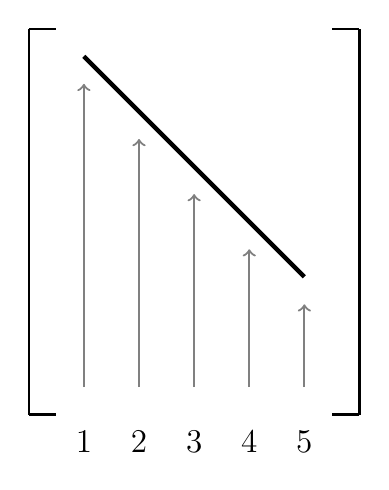
\begin{tikzpicture}[xscale=.7, yscale=.7]
\draw[->, gray, thick](0,0)--(0,5.5);
\draw[->, gray, thick](1,0)--(1,4.5);
\draw[->, gray, thick](2,0)--(2,3.5);
\draw[->, gray, thick](3,0)--(3,2.5);
\draw[->, gray, thick](4,0)--(4,1.5);
\node[draw=none] at(0,-1){\large 1};
\node[draw=none] at(1,-1){\large 2};
\node[draw=none] at(2,-1){\large 3};
\node[draw=none] at(3,-1){\large 4};
\node[draw=none] at(4,-1){\large 5};

\draw[-, ultra thick] (0,6)--(4,2);

\draw[-, thick](-1,-.5)--(-1,6.5);
\draw[-, thick](-1, -.5)--(-.5,-.5);
\draw[-, thick](-1,6.5)--(-.5,6.5);

\draw[-, thick](5,-.5)--(5,6.5);
\draw[-, thick](5,-.5)--(4.5,-.5);
\draw[-, thick](5,6.5)--(4.5,6.5);

%\draw[-, thick](-.5,0)--(3,0);
%\draw[-, thick](0,-.5)--(0,1.5);
%\draw[->, thick, >=stealth'](0,0)--(2.5,1);
%\draw[-,thick](2.5,-.2)--(2.5,.2);
%\draw[-, thick](-.2,1)--(.2,1);
%\node[draw=none](point_b)at(2.5,-.4){$a$};
%\node[draw=none](point_a)at(-.4,1){$b$};
%\draw[-, thick] (.5,.2)arc [start angle=60, 
%	end angle=-20, radius=4.5pt];
%\node[draw=none](theta)at(.8, .15){$\theta$};
\end{tikzpicture}
\caption{This figure illustrates the order in which to zero out subdiagonal entries in the Givens triangularization algorithm. 
The heavy black line is the main diagonal of the matrix. 
Entries should be zeroed out from bottom to top in each column, beginning with the leftmost column.}
\label{fig:givens}
\end{center}
\end{figure}


For example, on a $2 \times 3$ matrix we may perform the following operations:

\def\mc#1{\multicolumn{1}{c|}{#1}}
\def\lc#1{\multicolumn{1}{|c}{#1}}
\[
\begin{array}{ccccccc}
\begin{pmatrix}
*&*\\
*&*\\
*&*
\end{pmatrix}
&
\underrightarrow{G(2,3,\theta_1)}
&\begin{pmatrix}
&*&*&\\ \cline{2-3}
&\lc{*}&\mc{*}&\\
&\lc{0}&\mc{*}& \\ \cline{2-3}
\end{pmatrix}
&
\underrightarrow{G(1,2,\theta_2)}
& \begin{pmatrix} \cline{2-3}
&\lc{*}&\mc{*}&\\
&\lc{0}&\mc{*}&\\ \cline{2-3}
&0&*&
\end{pmatrix}
&
\underrightarrow{G(2,3,\theta_3)}
&\begin{pmatrix}
*&*&\\ \cline{2-2}
\mc{0}&\mc{*}&\\
\mc{0}&\mc{0}&\\ \cline{2-2}
\end{pmatrix}
\end{array}
\]
At each stage, the boxed entries are those modified by the previous transformation. 
The final transformation $G(2,3,\theta_3)$ operates on the bottom two rows, but since the first two entries are zero, they are unaffected. 
Assuming that at the $ij^{th}$ stage of the algorithm, $a_{ij}$ is nonzero, Algorithm \ref{Alg:givens} computes the Givens triangularization of a matrix..


\begin{algorithm}
\begin{algorithmic}[1]
\caption{Givens triangularization. Return an orthogonal matrix $Q$ and an upper triangular matrix $R$ satisfying $A = QR$.}
\label{Alg:givens}
\Procedure{Givens Triangularization}{$A$}
\State $m, n \gets \shape{A}$
\State $R \gets \makecopy{A}$
\State $Q \gets \Id{m}$
\State $G \gets \allocate{2}{2}$
\For{$j=0\ldots n-1$}
    \For{$i=m-1\ldots j+1$}
      \State $a, b \gets R[i-1,j], R[i,j]$
      \State $G \gets [[a, b],[-b,a]]/\sqrt{a^2+b^2}$
      \State $R[i-1:i+1, j:] \gets GR[i-1:i+1, j:]$
      \State $Q[i-1:i+1,:] \gets GQ[i-1:i+1,:]$
    \EndFor
\EndFor
\State \pseudoli{return} $Q\trp , R$
\EndProcedure
\end{algorithmic}
\end{algorithm}

Notice that in Algorithm \ref{Alg:givens}, we \emph{do not} actually create the matrices $G(i,j,\theta)$ and multiply them by the original matrix.
Instead we modify only those entries of the matrix that are affected by the transformation. As an additional way to save memory, it is possible to modify this algorithm so that $Q$ and $R$ are stored in the original matrix $A$.
\begin{comment}
An interesting side-note is that each Givens rotation can be represented as a single floating point number, so, when operating in place, $Q$ can be stored entirely in the lower triangular portion of the array on which we are operating by storing each rotation in the entry that it zeroes out.
A similar approach would to store Householder reflectors in the columns they zero out.
In either case, we can represent the QR decomposition of an array using only the memory that was originally used to store the array itself.
This is similar to the approach  for computing the LU decomposition entirely in place.
These representations of $Q$ and $R$ can be used in various ways to perform matrix multiplication by $Q$, $Q\trp$ and $R$ as needed.
\end{comment}







\begin{comment}
\begin{itemize}[$\bullet$]

\item Make $R$ a copy of $A$ and $Q$ an identity array of the appropriate size.

\item Make an empty $2 \times 2$ array $G$ that will be used to apply the Givens rotations.

\item For each column:

  \begin{itemize}[$\bullet$]

  \item For each row below the main diagonal (starting at the bottom of the column):

    \begin{itemize}[$\bullet$]

    \item If the leading entry of this row is not zero (i.e. if its absolute value is within a given tolerance):

      \begin{itemize}[$\bullet$]

      \item Compute $c$ and $s$ using the entry in the current row and column and the entry immediately above it.

      \item Use $c$ and $s$ to construct the matrix $G$.

      \item Get a slice of $R$ of the current row and the row above it that includes the columns from the current column onward.
      Multiply it in place by $G$ to zero out the leading nonzero entry of the current row.

      \item Get a slice of $Q$ of the current row and the row above it and apply $G$ to it as well. (Strictly speaking, you do not need to operate over these entire rows, but the slicing needed to avoid the extra computation is a little more involved, so we will not include that here.)

      \end{itemize}

    \end{itemize}

  \end{itemize}

\item Return $Q\trp$ and $R$.

\end{itemize}
\end{comment}


\begin{problem}
\label{prob:Givens}
(Optional)
Write a function that computes the Givens triangularization of a matrix, using Algorithm \ref{Alg:givens}. 
Assume that at the $ij^{th}$ stage of the algorithm, $a_{ij}$ will be nonzero.
\end{problem}


\begin{problem}
\label{prob:givens_hessenberg}
(Optional)
Modify your solution to Problem \ref{prob:Givens} to compute the Givens triangularization of an upper Hessenberg matrix, making the following changes:
\begin{enumerate}
\item Iterate through the first subdiagonal from left to right. (These are the only entries that need to be zeroed out.)
\item Line 11 of Algorithm \ref{Alg:givens} updates $Q$ with the current Givens rotation $G$. Decrease the number of entries of $Q$ that are modified in this line. Do this by replacing $Q[i-1:i+1, :]$ with $Q[i-1:i+1, :k_i]$ where $k_i$ is some appropriately chosen number (dependent on $i$) such that $Q[i-1:i+1, k_i:]=0$.
\end{enumerate}
Hint: Here is how to generate a random upper Hessenberg matrix on which to test your function.
The idea is to generate a random matrix and then zero out all entries below the first subdiagonal.
\begin{lstlisting}
import numpy as np
import scipy.linalg as la
from math import sqrt
A = np.random.rand(500, 500)

# We do not need to modify the first row of A
# la.triu(A[1:]) zeros out all entries below the diagonal of A[1:]
A[1:] = la.triu(A[1:])

# A is now upper Hessenberg
\end{lstlisting}

\begin{comment}
What is the computational order of  complexity for this problem?
Approximately for what $m$ is your implementation as fast as the general QR decomposition built in to \li{scipy.linalg} for computing the QR decomposition of an upper Hessenberg matrix?
\end{comment}
\end{problem}

\begin{comment}
\begin{problem}
\label{prob:givens_hessenberg_modified}
You may have noticed that matrix multiplication by $Q$ is generally a $\mathcal{O} \left( n^3 \right)$ algorithm, while the application of these individual Givens rotations is a $\mathcal{O} \left( n^2 \right)$ algorithm.
Write a modified version of your solution to Problem \ref{prob:givens_hessenberg} called \li{givens2_mod} which returns 
an $(n-1) \times 2 \times 2$ array containing the computed values for $G$ at each step in the algorithm in the order in which they are applied to the upper Hessenberg array $H$.

Write two more functions \li{apply_Q} and \li{apply_QT} which, using the matrix of Givens rotations, perform left multiplication 
by $Q$ and $Q^{-1}$, respectively, on some other input array $B$.
Left multiplication by $Q^{-1}$ can be done by applying each of the Givens rotations to $B$ the same way you did to $H$ to compute its QR factorization.
Left multiplication by $Q$ can be done by applying the transpose of the Givens rotations to their corresponding portions of $B$, but in the reverse order.
Notice that you will have to apply each Givens rotation across the full width of the rows it operates on since you do not know anything about the content of $B$.

For around what size of matrices is direct multiplication by $Q$ slower than this method of multiplying by $Q$?
For timing purposes, make a random upper Hessenberg matrix, compute its QR decomposition using the function you just wrote and your solution to Problem \ref{prob:givens_hessenberg}, then time how long it takes to left multiply a random square array by $Q$ using the function you just wrote and the \li{dot} method of NumPy arrays.

Note: the functions you just wrote can be used to perform right multiplication as well since $B Q = \left(Q\trp B\trp \right)\trp$ and $B Q\trp = \left( Q B\trp \right)\trp$.
\end{problem}
\end{comment}

%Sources: http://www.cs.unc.edu/~krishnas/eigen/node5.html
% http://en.wikipedia.org/wiki/Givens_rotation
%http://en.wikipedia.org/wiki/QR_decomposition
%	Note the Operation count: Householder is 2/3 n^3, MGS is 2 n^3
%http://en.wikipedia.org/wiki/QR_algorithm
%Applied Numerical methods using MATLAB by Yang has some code written for this
%http://www.math.kent.edu/~reichel/courses/intr.num.comp.2/lecture21/evmeth.pdf
%	These are eigenvalue algorithms explained carefully
%http://en.wikipedia.org/wiki/Householder_transformation
%Numerical Linear Algebra, by Lloyd N. Trefethen and David Bau III, Chapters 10 and 16 

